\chapter[Chapter 1]{Complex Analysis}

\section{Complex Numbers $\mathbb C$}
\subsection{Imaginary unit}
We define $i$ to be the imaginary unit, such that $i^2=-1$. Any complex number can be decomposed into two parts:
$$
z=x+yi\qquad x,y\in\mathbb R
$$
where $x=\operatorname{Re}(z)$ and $y=\operatorname{Im}(z)$.

We can see many similarities of $\mathbb C$ and $\mathbb R^2$.

\subsection{Complex Conjugate}
We define the Complex conjugate $\overline z$ as: 
$$
\overline z = x-yi
$$
\begin{figure}[H]
    \begin{center}
    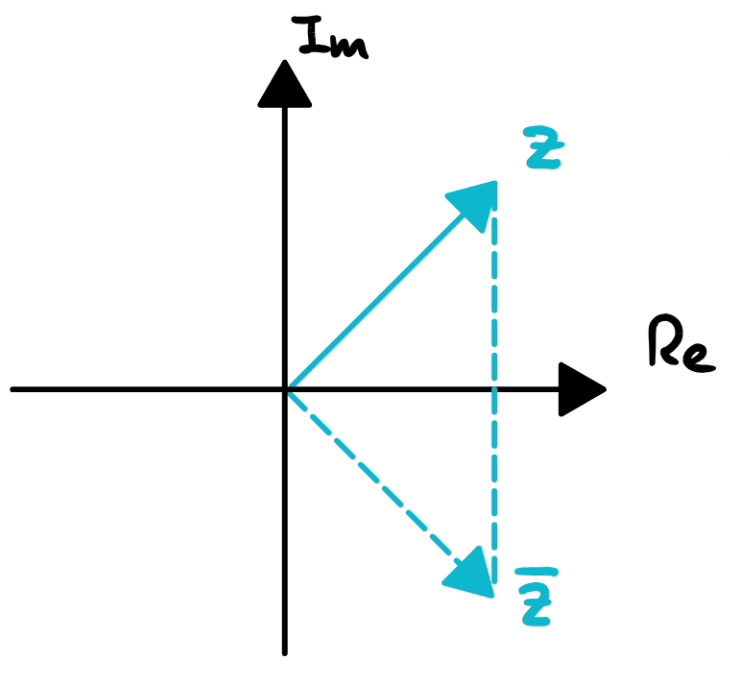
\includegraphics[width=0.4\textwidth]{ComplexConjugate.png}
    \caption{plot real and imaginary part with complex conjugate as vectors}
    \end{center}
\end{figure}

\subsection{Modulus (Absolute Value)}
We define the modulus to be
$$
\lvert z \rvert = \sqrt{x^2+y^2}
$$
If $z_0,z_1\in\mathbb C$, then the distance between the two points can be described by $\lvert z_1-z_0\rvert$.


\subsection{Euler's Formula}
For $\theta\in \mathbb R$: 
$$
e^{i\theta} = \cos\theta + i\sin\theta
$$

\begin{figure}[H]
    \begin{center}
    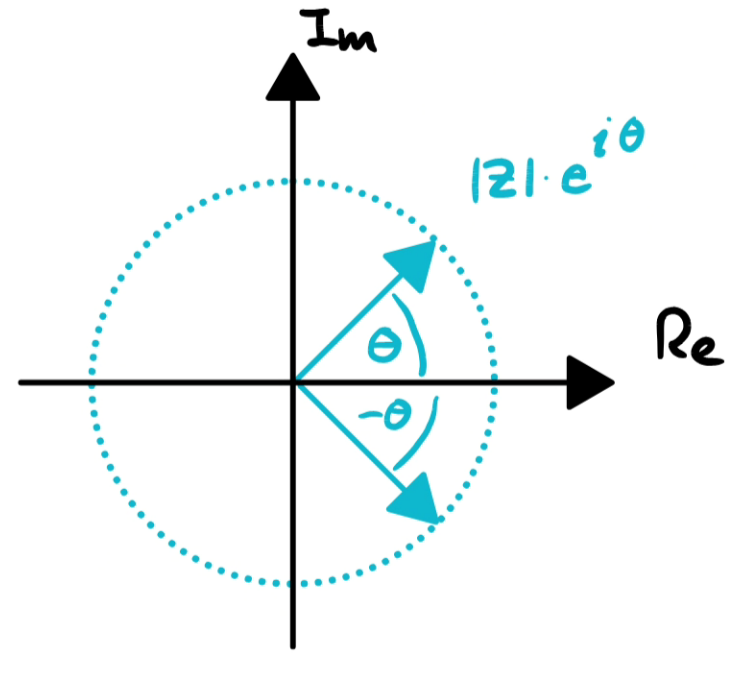
\includegraphics[width=0.4\textwidth]{PolarExpression.png}
    \caption{plot with circle showcasing $e^{i\theta}$, similar to polar coordinates}
    \end{center}
\end{figure}

 
This yields the observations:
\begin{itemize}
    \item $\lvert e^{i\theta}\rvert = 1$
    \item $\overline{\lvert e^{i\theta}\rvert} = \rvert e^{-i\theta}\rvert$
\end{itemize}

\subsubsection{Algebraic Operations}
with two imaginary numbers $z_1=x_1+iy_1, z_2=x_2+iy2$ the basic operations are as follows:
\begin{itemize}
    \item {Addition} $z_1\pm z_2 = (x_1\pm x_2) + i(y_1\pm y_2)$
    \item {Multiplication} $z_1\cdot  z_2 = (x_1 + iy_1) \cdot  (x_2+i y_2) = (x_1x_2-y_1y_2)+i(x_1y_2+x_2y_1)$
    \item {Multiplication with complex conjugate} $z\cdot \overline z = \lvert z\rvert ^2$
\end{itemize}
Note that multiplication with the complex conjugate can be useful for expanding fractions: 
$$
\frac{z_1}{z_2}=\frac{z_1\overline{z_2}}{\lvert z_2\rvert ^2}
$$

\subsection{Polar expression}
For complex numbers $z_n=\lvert z\rvert \cdot e^{i\theta}$ to be the same, we need:

\begin{equation*}
z_1=z_2
\Rightarrow 
\begin{cases}
|z_1|=|z_2|\\
\theta_1-\theta_2 \in 2\pi \mathbb Z
\end{cases}
\end{equation*}
\subsubsection{Principal Argument}
$$
\operatorname{Arg}(z)\in[-\pi,+\pi]\implies z= |z| \cdot e^{i\operatorname{Arg}(z)}
$$

\subsubsection{Algebraic Operations}
With the polar expression multiplication of two complex numbers yields:
\begin{equation*}
\begin{split}
    z_1\cdot z_2 &= |z_1||z_2|e^{i(\theta_1+\theta_2)}\\
    \frac{z_1}{z_2} &= \frac{|z_1|}{|z_2|}e^{i(\theta_1-\theta_2)} 
\end{split}
\end{equation*}

We can conclude that if $x=0, \theta =\pm\pi/2$ and if $x\ne 0, \theta = \arctan\frac yx$.

\subsection{Examples}
To solve $z^5=2$ for $z$, we use the polar expression:
\begin{equation*}
\begin{split}
|z|^5 \cdot e^{i5\operatorname{Arg}(z)}=2&=2\cdot e^{i0}\\
&\implies
\begin{cases}
    \operatorname{Arg}(z) \in \frac 25\pi \mathbb Z\\
    \operatorname{Arg}(z) \in]-\pi,\pi]
\end{cases}\\
&\implies
\operatorname{Arg}(z)\in\left\{-\frac{4\pi}5,-\frac{2\pi}5 , 0, \frac{2\pi}5, \frac{4\pi}{5}\right\}
\end{split}
\end{equation*}

\section{Complex Functions}
A complex function $f: \mathbb C \to\mathbb C$ is a function that takes a complex variable and returns another complex number that can be decomposed into a real and imaginary parts. We can therefore think of them as two functions, $u, v: \mathbb R^2 \to \mathbb R$:
\begin{equation*}
\begin{split}
z:x+iy\to f(z)=u(x,y)+i\cdot v(x,y)
\end{split}
\end{equation*}

\subsection{Important Complex Functions}
\begin{itemize}
    \item $f(z)=z=x+yi$
    \item $f(z)=\overline z=x-yi$
    \item $f(z)=z^2=x^2-y^2+2xyi$
    \item $f(z)=e^z=e^{x+iy}=e^x=e^x(\cos y+i\sin y)=e^x\cos y + i(e^x\sin y)$
    \item $\cos(z)=\frac{e^{iz}+e^{-iz}}2$
    \item $\sin(z)=\frac{e^{iz}-e^{-iz}}2$
    \item $\cosh(z)=\frac{e^z+e^-i}{2}$
    \item $\sinh(z)=\frac{e^z-e^-i}{2}$
\end{itemize}
\textbf{Note:} The complex exponent function $\exp$ here is assumed to behave exactly as it would with real functions.

As an example, we can try to find the real and imaginary parts of the cosine function:
\begin{equation*}
\begin{split}
\cos(z)&=\cos(x+yi)\\
&=\frac{e^{i(x+yi)}+e^{-i(x+yi)}}2\\
&=\frac 12 \left(e^{-y}e^{ix}+e^ye^{-ix}\right)\\
&=\frac 12(e^{-y}+e^y)\cos x + \frac i2 (e^y-e^y)\sin x\\
&=\cosh y\cdot \cos x + i \sinh y \sin x
\end{split}
\end{equation*}
Which is an important identity.

\subsection{Definition: Limits and continuity}
We will say that $z_n\stackrel{n}{\rightarrow}z_0$ 
if for any $\varepsilon > 0$, there exists $N > 0$ such that  for any $n > N$, $|z_n-z_0| < \varepsilon$, $\lim_{n\to +\infty} z_n = z_0$.

Let $f:\mathbb C \to \mathbb C$ and $z_0\in \mathbb C$. We will say that $f$ is continuous at $z_0$ if for any $\varepsilon > 0 $, there exists a $\delta > 0$ such that when $|z-z_0| < \delta\implies |f(z)-f(z_0)| < \varepsilon$.
Equivalently, $\lim_{z\to z_0} = f(z_0)$.

Let $f(x+yi) = u(x,y)+iv(x,y)$. $f$ is continuous at $z_0=x_0+y_0i\Leftrightarrow$ $u$ and $v$ are continuous at $(x_0,y_0)$.

$f$ is continuous at a point $z_0\Leftrightarrow$ for every sequence $z_n\stackrel{n\to\infty}\to z_0$ the images converge: $f(z_n)\stackrel{n\to\infty}\to f(z_0)$ 

\subsection{Differentiability, Holomorphic and Entire Functions}
Let $f:\mathbb C \to\mathbb C$ be a complex function. We will say that $f$ is (complex) differentiable at $z_0$ if the limit $$\lim_{z\to z_0} \frac{f(z)-f(z_0)}{z-z_0}$$ exists, is finite, and is denoted by $f'(z_0)$.

\begin{itemize}
    \item if $f$ is differentiable at every point of an open set $W$ then $f$ is \textbf{holomorphic} on $W$.
    \item if $f$ is holomorphic on $\mathbb C$ then $f$ is \textbf{entire}.
\end{itemize}
\textbf{Reminder:} A set $W\subseteq \mathbb C$ is open if $\forall z_0 \in W\exists \varepsilon > 0$ such that $D=\{z:|z-z_0|<\varepsilon\}\subseteq W$.

\subsubsection{Examples}
To differentiate $f(z)=z$ at $z_0$ we take the limit:
$$
f'(z_0) = \lim_{z\to z_0} \frac{z-z_0}{z-z_0} = 1
$$
When differentiating $f(z)=1/z$ on $\mathbb C^\ast$ we get that $$f'(z)=-\frac 1{z^2}$$ Which shows that $f$ is holomorphic on $\mathbb C^\ast$.

\subsubsection{Properties}
\begin{itemize}
    \item If $f$,$g$ are continuous / differentiable at $z_0$ then the same is true for $f+g$ and $f\cdot g$.
    \item Derivative of a product and of compositions are the same as on $\mathbb{R}$.
\end{itemize}

\subsection{Cauchy-Riemann Equations}
Let $f:\mathbb C \to\mathbb C, f(x+yi)=u(x,y)+v(x,y)i$. 
Then the two statements are equivalent:
\begin{itemize}
    \item $f$ is complex differentiable
    \item $u,v$ have continuous derivatives and satisfy
    \begin{equation*}
        \begin{split}
            u_x&=v_y\\
            u_y&=-v_x
        \end{split}
    \end{equation*}
\end{itemize}



